\documentclass[letterpaper,12pt]{article}

\usepackage{ucs}
\usepackage[utf8x]{inputenc}
\usepackage{amsmath}
%\usepackage{amsfonts}
%\usepackage{amssymb}
\usepackage[margin=1in]{geometry}
\usepackage{graphicx}
\usepackage[bitstream-charter]{mathdesign}
\usepackage[T1]{fontenc}

\newcommand{\len}[1]{\lVert #1\rVert}
\newcommand{\abs}[1]{\lvert #1\rvert}
\newcommand{\R}{\mathbb{R}}
\title{Math 1410 Assignment \#1 Solutions\\University of Lethbridge, Spring 2017}
\author{Sean Fitzpatrick}
\begin{document}
 \maketitle


\begin{enumerate}
\item Prove the \textit{distributive property} for complex arithmetic. That is, prove that for any complex numbers $u, v, w$, we have
\[
 u(v+w) = uv+uw.
\]

\medskip

{\bf Solution:} Let $u=a+ib$, $v=c+id$, and $w=e+if$ be arbitrary complex numbers, where $a,b,c,d,e,f\in\R$. Then we have
\begin{align*}
 u(v+w) & = (a+ib)[(c+id)+(e+if)]\\
& = (a+ib)[(c+e)+i(d+f)]\\
& = [a(c+e)-b(d+f)]+i[(b(c+e)+a(d+f)] \tag{using $i^2=-1$}\\
& = (ac+ae-bd-bf)+i(bc+be+ad+af)\\
& = [(ac-bd)+i(bc+ad)]+[(ae-bf)+i(be+af)] \tag{rearranging}\\
& = [(a+ib)(c+id)]+[(a+ib)(e+if)] \tag{reversing the definition of complex multiplication}\\
& = uv+uw,
\end{align*}
as required.

\bigskip

\item Recall that the complex conjugate of $z\in\mathbb{C}$ is denoted by $\overline{z}$, and the modulus of $z$ is denoted by $\abs{z}$. Show that:
\begin{enumerate}
 \item $\abs{\overline{z}} = \abs{z}$
 \item $\abs{z} = \sqrt{z\overline{z}}$
 \item $\operatorname{Re}(z) = \dfrac{z+\overline{z}}{2}$ and $\operatorname{Im}(z) = \dfrac{z-\overline{z}}{2i}$, where $\operatorname{Re}(z)$ and $\operatorname{Im}(z)$ denote the real and imaginary parts of $z$, respectively.
\end{enumerate}

\bigskip

{\bf Solution:} Let $z=x+iy$, where $x,y\in \R$, be any complex number. Then:
\begin{enumerate}
 \item Since $\overline{z}=x-iy=x+i(-y)$ by definition of the complex conjugate, the modulus formula gives us
\[
 \abs{\overline{z}} = \sqrt{x^2+(-y)^2} = \sqrt{x^2+y^2} = \abs{z}.
\]
 \item Using the rules for complex multiplication, we have
\[
 z\overline{z} = (x+iy)(x-iy) = x^2-ixy+ixy-i^2y^2 = x^2+y^2.
\]
It follows that $\abs{z} = \sqrt{x^2+y^2} = \sqrt{z\overline{z}}$.
 \item By definition, with $z=x+iy$ we have $\operatorname{Re}(z) = x$ and $\operatorname{Im}(z)=y$. We can then verify that
\[
 \frac{z+\overline{z}}{2} = \frac{(x+iy)+(x-iy)}{2} = \frac{2x}{2} = x = \operatorname{Re}(z),
\]
and
\[
 \frac{z-\overline{z}}{2i} = \frac{(x+iy)-(x-iy)}{2i} = \frac{2iy}{2i} = y = \operatorname{Im}(z).
\]

\end{enumerate}

\medskip

\item Convert $z=-1+\sqrt{3}i$ to polar form, and compute the value of $z^6 = (-1+\sqrt{3}i)^6$. Express your answer in rectangular form.

\medskip

{\bf Solution:} We compute $\abs{z} = \sqrt{(-1)^2+(\sqrt{3})^2} = \sqrt{1+3} = 2$, and thus
\[
 z = 2\left(-\frac{1}{2}+i\frac{\sqrt{3}}{2}\right) = 2\left(\cos\left(\frac{2\pi}{3}\right)+i\sin\left(\frac{2\pi}{3}\right)\right) = 2e^{i(2\pi/3)}.
\]
It follows that
\[
 z^6 = (2e^{i(2\pi/3)})^6 = 2^6e^{i\cdot 6(2\pi/3)} = 2^6e^{i(4\pi)} = 64(\cos(4\pi)+i\sin(4\pi)) = 64.
\]

\bigskip

\item  Let $\vec{v} = \langle 3, -1, 4\rangle$ and $\vec{w} = \langle -2, 5, 1\rangle$ be two vectors in $\R^3$. Find the coordinates of:
\begin{enumerate}
 \item The point $P$, one half of the way from the tip of $\vec{v}$ to the tip of $\vec{w}$.

\medskip

{\bf Solution:} Referring to the diagram below, we see that the vector $\vec{v}-\vec{w}$ (when drawn with its tail at the tip of $\vec{w}$), points all the way from the tip of $\vec{w}$ to the tip of $\vec{v}$. We want the point $P$ (as marked) that is half-way between these two points; this can be achieved by adding one half of the vector $\vec{v}-\vec{w}$ to $\vec{w}$. Thus, the position vector for $P$ is given by
\begin{align*}
 \overrightarrow{OP} & = \vec{w}+\frac{1}{2}(\vec{v}-\vec{w})\\
 & = \frac{1}{2}\vec{v}+\frac{1}{2}\vec{w} = \frac{1}{2}(\vec{v}+\vec{w})\\
 & = \frac{1}{2}(\langle 3,-1,4\rangle + \langle -2,5,1\rangle)\\
 & = \frac{1}{2}\langle 1, 4, 5\rangle = \left\langle \frac{1}{2}, 2,\frac{5}{2}\right\rangle.
\end{align*}

\medskip

 \item The point $Q$, one third of the way from the tip of $\vec{v}+\vec{w}$ to the tip of $\vec{v}-\vec{w}$.

\medskip

{\bf Solution:} Again referring to our diagram, we see that if we draw the vector $\vec{v}-\vec{w}$ with its tail at the origin, then the vector $\vec{w}+\vec{w} = 2\vec{w}$ points all the way from the tip of $\vec{v}-\vec{w}$ to the tip of $\vec{v}+\vec{w}$. We want the point $Q$ that is one-third of the way {\em from} the tip of $\vec{v}+\vec{w}$ {\em to} the tip of $\vec{v}-\vec{w}$. If we are starting at the tip of $\vec{v}+\vec{w}$ and ending at the tip of $\vec{v}-\vec{w}$, then we are moving opposite to the vector $2\vec{w}$, so we need to use $-2\vec{w}$. However, we only want to go one third of the way, which tells us that we should add the vector $\frac{1}{3}(-2\vec{w}) = -\frac{2}{3}\vec{w}$ to the vector $\vec{v}+\vec{w}$, according to the tip-to-tail rule for vector addition. Thus, we have
\begin{align*}
 \overrightarrow{OQ} & = (\vec{v}+\vec{w})+\left(-\frac{2}{3}\vec{w}\right)\\
& = \vec{v}+\frac{1}{3}\vec{w}\\
& = \langle 3, -1, 4\rangle +\frac{1}{3}\langle -2, 5, 1\rangle\\
& = \langle 3, -1, 4\rangle +\left\langle -\frac{2}{3}, \frac{5}{3}, \frac{1}{3}\right\rangle\\
& = \left\langle \frac{7}{3}, \frac{2}{3}, \frac{13}{3}\right\rangle.
\end{align*}
\begin{center}
 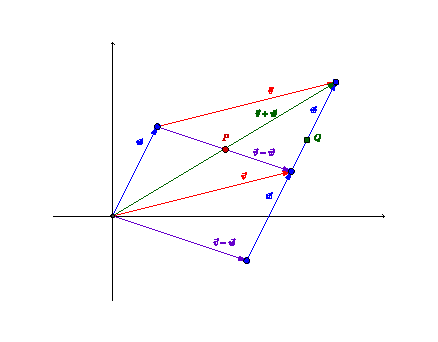
\includegraphics[width=6in]{A1_Q4}
\end{center}


\end{enumerate}

\end{enumerate}

\end{document}
 
